\documentclass[compress,red]{beamer}

\mode<presentation> {
	\usetheme{Warsaw}
}

%\beamertemplateballitem
\beamertemplateshadingbackground{gray!15}{white!15}
%\usecolortheme{crane}

% Import innych pakietow
\usepackage[utf8x]{inputenc}
\usepackage[MeX]{polski}
\usepackage{graphicx} 
\usepackage{listings}
\usepackage{amsmath}
\usepackage{amsfonts}
\usepackage{amssymb}
\usepackage{subfig}
\usepackage{verbatim}
\usepackage{algorithmic}		% Pseudokod
\usepackage{algorithm}

% USTAWIENIA PAKIETU LISTINGS
\lstloadlanguages{C}
\lstset{%
	language=C,% 
	numbers=none,%
	tabsize=4,%
	frame=single,%
	breaklines=true%
	}

% FullScreen w PDF'ach
%\hypersetup{pdfpagemode=FullScreen}


% Autor, Tytul itp.

\author{Marcin Chwedczuk \and Gleb Peregud}

\title{%
Całkowanie numeryczne
}

\institute{%
Wydział Matematyki i Nauk Informacyjnych\\
Politechnika Warszawska
}

\date{29 Listopad 2011}


%
% Głębokość spisu tresci
%
%\setcounter{tocdepth}{1} 

% Dodaj table of contents na poczatek 
% kazdej SUBsekcji
%\AtBeginSection[]
%{
%  \begin{frame}<beamer>{Agenda}
%    \tableofcontents[currentsection,currentsubsection]
%  \end{frame}
%}

% Poczatek prezentacji

\begin{document}
    \begin{frame}
        \titlepage
    \end{frame}

	\begin{frame}{Agenda}
		\tableofcontents
	\end{frame}

\section{Wstęp}

	\begin{frame}
		\frametitle{Wstęp}
		\only<1> { 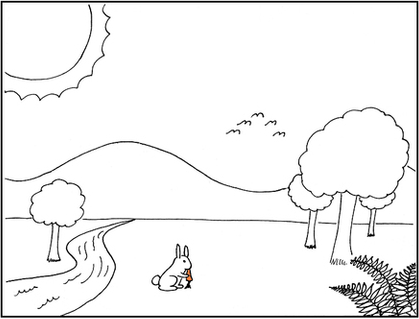
\includegraphics[scale=0.7]{./img/plain_world} }
		\only<2> { 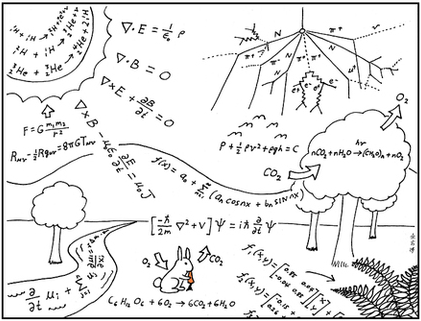
\includegraphics[scale=0.7]{./img/scientist_world} }
	\end{frame}

\section{Zakończenie}

	\begin{frame}
		\frametitle{Zakończenie}
		\only<1>{		
		\begin{Huge}
			Pytania ?
		\end{Huge}}
		\only<2>{
		\begin{Huge}
			Dziękuję za uwagę
		\end{Huge}
			}
	\end{frame}

\end{document}
